\section{TensorFlow Lite per Android}
TensorFlow Lite dispone di ambienti di esecuzione predefiniti e personalizzabili per l’esecuzione rapida e efficiente di modelli Android, incluse le opzioni per l'accelerazione hardware.

Come possiamo \textbf{eseguire un modello su Android}? Un modello TensorFlow Lite, all’interno di un’app Android, acquisisce ed elabora dati, generando una previsione basata sulla logica dello stesso modello.
Per essere eseguito, il modello ha bisogno di uno specifico ambiente di runtime e i dati di ingresso devono essere nel formato speciale tensor. Quando il modello esegue un’inferenza, produce risultati di
previsione nel formato tensor e li consegna all’app Android che, a seconda degli output ricevuti, intraprende una o più azioni (come mostrare a schermo il risultato o eseguire specifiche operazioni di calcolo).

\begin{figure}[ht]
    \centering
    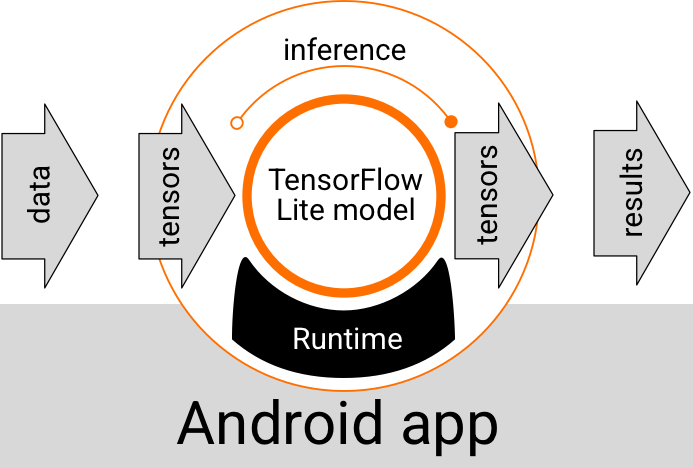
\includegraphics[width=0.6\textwidth]{Immagini/esecuzione.png}
    \caption{Schema di esecuzione di un modello in un app Android.}
    \label{fig:esecuzione}
\end{figure}

L’app, quindi, ha bisogno dei seguenti elementi per utilizzare un modello TF Lite:
\begin{itemize}
    \item Ambiente di runtime: per l’esecuzione del modello;
    \item Modellatore di input: per convertire i dati di ingresso nel formato textit{tensor};
    \item Modellatore di output: per ricevere i tensor di output e interpretarli come risultati di previsione.
\end{itemize}

\subsection{Ambiente di runtime}
Per l’esecuzione di un modello TensorFlow Lite su un app android c’è bisogno di un ambiente di runtime il quale può essere abilitato nei seguenti modi:
\begin{itemize}
    \item Google play services.
    \item Ambiente di runtime TensorFlow Lite Stand-alone.
\end{itemize}

Utilizzare i servizi Google Play è l’approccio preferito e consigliato. Infatti, questo ambiente di runtime è più efficiente in termini di spazio poiché si carica in modo dinamico, riducendo le dimensioni dell’app.
I servizi Google Play, inoltre, utilizzano automaticamente la versione più recente e aggiornata del runtime di TensorFlow Lite, offrendo funzionalità aggiuntive e prestazioni in continuo miglioramento. 
Adottare un ambiente di runtime fornito da Google Play Services ha degli svantaggi: il set di delegati per l’accelerazione hardware da cui si può scegliere si riduce e non sono supportate API TensorFLow Lite sperimentali
(come le operazioni personalizzate). Nel caso in cui i servizi Google Play non siano inclusi nell’app o nel caso in cui lo sviluppatore debba gestire il proprio modello machine learning “da vicino”, allora è conveniente usare
l’ambiente runtime TensorFlow Lite stand-alone che aggiunge codice nell’app, garantendo allo sviluppatore un maggiore controllo del runtime di machine learning al costo di un incremento della dimensione dell’app. 
Entrambi gli ambienti di runtime possono essere acceduti utilizzando specifiche API e librerie di sviluppo all’app.

\subsection{API e librerie di sviluppo}
Per integrare i modelli TensorFlow Lite in un applicazione Android, è possibile utilizzare due API molto utili fornite da TensorFlow Lite stesso:
\begin{itemize}
    \item L’API TensorFlow Lite Task;
    \item L’API TensorFLow LIte Interpreter.
\end{itemize}

Quali sono le differenze? L’API Interpreter fornisce classi e metodi per eseguire inferenze su modelli TensorFlow Lite già esistenti mentre L’API Task racchiude l’API Interpreter in un wrap che dispone di un’interfaccia
di programmazione ad alto livello per la gestione di attività di machine learning riguardo a dati visivi, audio e testuali. L’API Task viene sempre utilizzata nello sviluppo di applicazioni AI mobile, salvo casi specifici
in cui il dispositivo non è in grado di supportare tale API. Entrambe le API possono essere accedute tramite i servizi di Google Play.

\subsection{I tensori}
Al fine di comprendere maggiormente la prossima sezione, è giusto approfondire il concetto di tensore. Un tensore è un array multidimensionale con un tipo uniforme (chiamato dtype, o data type) di cui vettori, matrici, funzioni
lineari ed endomorfismi costituiscono casi particolari. Tutti i tensori sono immutabili: non è mai possibile modificare il contenuto di un tensore, solamente crearne uno nuovo (a eccezione del caso specifico dei tensori di tipo tf.Variable).
Oltre al data type, i tensori possiedono due caratteristiche principali: la forma (o shape), ossia la lunghezza di ogni dimensione, e il grado (o rank) che consiste nel numero di dimensioni del tensore e può essere considerato
il suo ordine di grandezza.

Per esempio, uno scalare è un tensore di rank 0 e di shape nulla, un vettore è un tensore di rank 1 e di shape che corrisponde al numero di elementi del vettore, una matrice è un tensore di rank 2 (2 dimensioni) e di shape costituita
da due numeri: il numero di righe e il numero di colonne.

Al fine di creare un rete neurale, si utilizzano delle rappresentazioni grafiche per mostrare il flusso di calcolo dei dati e le operazioni avvenute. Per fare ciò, si utilizza un grafo: la rappresentazione, per mezzo di nodi,
di operazioni eseguite sui tensori. Il grafo è costituito da nodi che rappresentano i tensori e i dati memorizzati all’interno di essi e da nodi che rappresentano le operazioni su tali dati. I tensori si uniscono tra di loro
per formare unità neurali più complesse, come il percettrone.

Una rete neurale è costituita da innumerevoli percettroni, caratterizzando la complessità del mondo AI. Dopo questa brevissima introduzione dei tensori, torniamo a TensorFlow Lite che, come suggerisce il nome, sfrutta a pieno
la struttura dati appena introdotta.

\begin{figure}[ht]
    \centering
    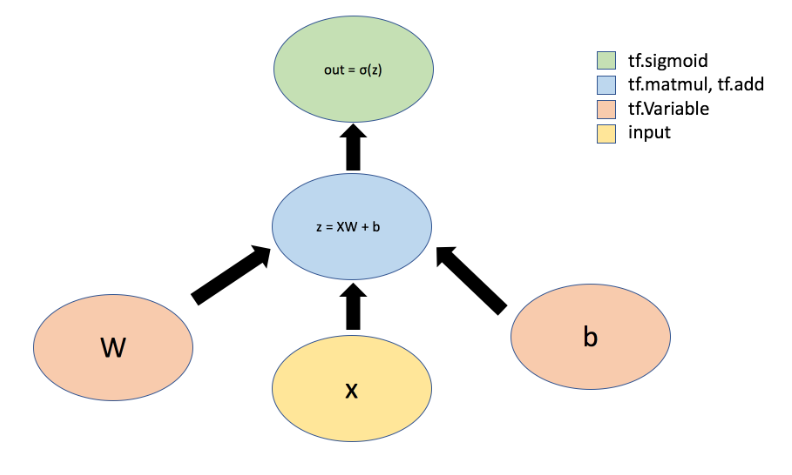
\includegraphics[width=0.7\textwidth]{Immagini/tensore.png}
    \caption{Percettrone, esempio di un semplice grafo con tensori e operazioni}
    \label{fig:tensore}
\end{figure}

\newpage
\section{Gestione dei dati in input}
Come già anticipato, per elaborare i dati di input è necessario che essi siano nel formato di tensore. Il tensore, inoltre, deve essere in una specifica forma. Ogni modello TensorFlow Lite di machine learning, quindi, deve trasformare
un dato in input dal suo formato nativo (immagine, testo, audio…) in un tensore con la specifica forma richiesta dal modello. Molto spesso il formato richiesto viene specificato nei metadati del modello. Come eseguire tale trasformazione?
TensorFlow Lite fornisce una libreria apposita chiamata TensorFlow Lite Task che dispone di una logica di gestione dati per la conversione dei dati da un qualsiasi formato a un tensore con la forma giusta.

Una volta ottenuto un ambiente di runtime ottimale, un modello e dei dati di input nel formato richiesto è possibile eseguire inferenze come descritto precedentemente nel report.

\section{Gestione dei risultati in output}
Eseguita l’inferenza, il modello produce in output dei risultati nella forma di tensori che devono essere gestiti ed interpretati dall’applicazione android agendo o mostrando a schermo un risultato per l’utente. 
I tensori di output possono essere dei semplici numeri che corrispondono ad un singolo risultato (per esempio, 0 = gatto, 1 = cane, 2 = pesce) per una classificazione di immagini, ma possono essere anche risultati estremamente
complessi come diversi riquadri di delimitazione nel caso in cui vi siano più oggetti classificati in un’immagine, insieme a delle valutazioni di affidabilità delle previsioni nell’intervallo [0, 1].

Molto spesso la descrizione dei risultati di output e di come interpretarli viene fornita dai metadati incorporati nel modello.

\section{Approcci di sviluppo avanzati}
Nel caso in cui vengano utilizzati modelli TensorFlow Lite più sofisticati, potrebbe essere necessario utilizzare percorsi di sviluppo avanzati e più complicati rispetto a quanto descritto sopra. Quindi,
si utilizzano delle tecniche avanzate per sviluppare ed eseguire modelli TensorFlow LIte in un’app Android:
\begin{itemize}
    \item Ambiente di runtime avanzato: quando si dispone di un modello di machine learning che utilizza operazioni non supportate dall’ambiente di runtime standard di TensorFlow Lite o da quello fornito dai servizi di Google Play,
    è possibile utilizzare degli ambienti runtime avanzati: l’ambiente runtime TensorFlow Lite Flex, che permette di implementare operatori specifici per il proprio modello el’ ambiente runtime TensorFlow Lite personalizzato.
    Come opzione ancora più avanzata, è possibile importare la libreria TensorFlow Lite su Android per l’inclusione di funzionalità e operatori richiesti per eseguire il proprio modello.
    \item APIs di C e C++: TensorFlow Lite fornisce delle API per eseguire modelli usando C e C++. L’utilizzo di queste API è consigliato quando l’applicazione usa Android NDK o se si vuole condividere codice tra piattaforme.
    \item Esecuzione del modello su un server: l’esecuzione dei modelli nella propria app Android permette di abbassare la latenza e migliorare la privacy per gli utenti. In alcuni casi, però, conviene eseguire il proprio modello
    su un server cloud: per esempio, questo approccio è consigliato se il modello è troppo grande e non è facilmente comprimibile in una dimensione gestibile da dispositivi Android degli utenti. Inoltre, si utilizza questa tecnica
    quando è prioritario garantire una performance consistente del modello su un vasto range di dispositivi.
    \item Ottimizzazione di modelli personalizzati: è importante considerare di ottimizzare il proprio modello personalizzato per ridurre costi di elaborazione e di memoria. L’approccio consigliato è sempre quello della quantizzazione. 
\end{itemize}